% Asset ID: A21BinomialExpansionTikZ-004
% Unit: A21
% Topic code: A21-SS
% Topic ID: A21BinomialExpansion
% Purpose: Combining expansions power tracking
\documentclass[tikz,border=10pt]{standalone}
\usepackage{amsmath}
\usetikzlibrary{arrows.meta,positioning}
\begin{document}
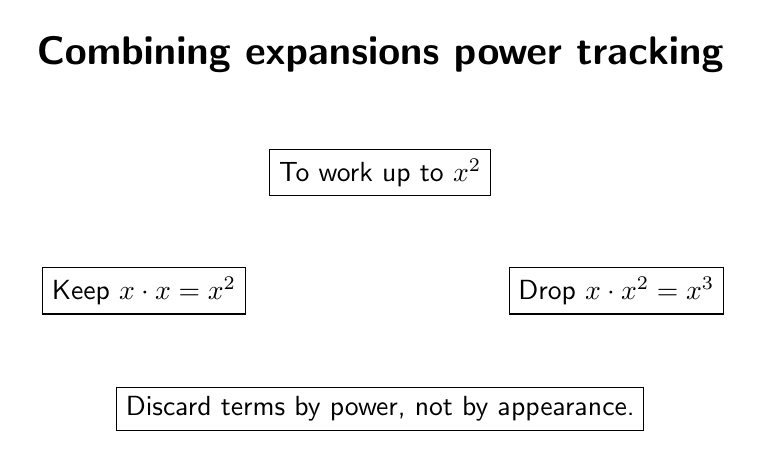
\begin{tikzpicture}[every node/.style={font=\sffamily}]
\node[font=\sffamily\bfseries\Large] at (0,3) {Combining expansions power tracking};
\node[draw,align=center] at (0,1.5) {To work up to $x^2$};\node[draw,align=center] at (-3,0) {Keep $x\cdot x=x^2$};\node[draw,align=center] at (3,0) {Drop $x\cdot x^2=x^3$};\node[draw,align=center] at (0,-1.5) {Discard terms by power, not by appearance.};
\end{tikzpicture}
\end{document}
